\documentclass{standalone}
\usepackage{tikz}
\usetikzlibrary{patterns, positioning}

\begin{document}
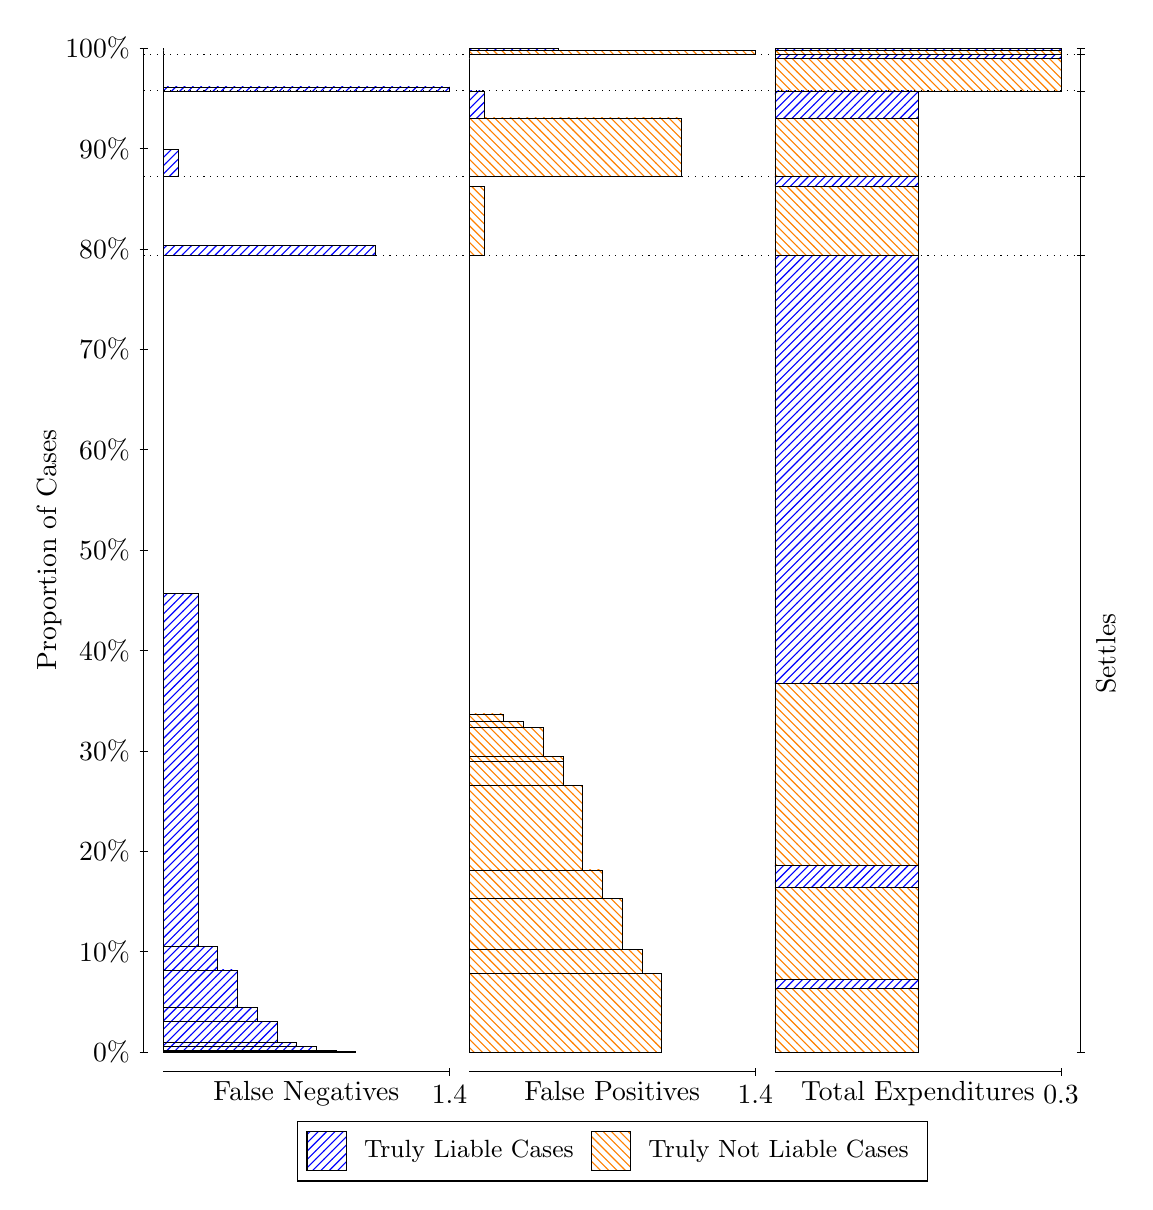
\begin{tikzpicture}
\draw[black, very thin] (1.5,1.75) -- (1.5,14.5);
\node[rotate=90, anchor=center] at (0.3, 8.125) {Proportion of Cases};
\draw[black, very thin] (1.45,1.75) -- (1.55,1.75);
\node[anchor=east] at (1.45, 1.75) {0\%};
\draw[black, very thin] (1.45,3.025) -- (1.55,3.025);
\node[anchor=east] at (1.45, 3.025) {10\%};
\draw[black, very thin] (1.45,4.3) -- (1.55,4.3);
\node[anchor=east] at (1.45, 4.3) {20\%};
\draw[black, very thin] (1.45,5.575) -- (1.55,5.575);
\node[anchor=east] at (1.45, 5.575) {30\%};
\draw[black, very thin] (1.45,6.85) -- (1.55,6.85);
\node[anchor=east] at (1.45, 6.85) {40\%};
\draw[black, very thin] (1.45,8.125) -- (1.55,8.125);
\node[anchor=east] at (1.45, 8.125) {50\%};
\draw[black, very thin] (1.45,9.4) -- (1.55,9.4);
\node[anchor=east] at (1.45, 9.4) {60\%};
\draw[black, very thin] (1.45,10.675) -- (1.55,10.675);
\node[anchor=east] at (1.45, 10.675) {70\%};
\draw[black, very thin] (1.45,11.95) -- (1.55,11.95);
\node[anchor=east] at (1.45, 11.95) {80\%};
\draw[black, very thin] (1.45,13.225) -- (1.55,13.225);
\node[anchor=east] at (1.45, 13.225) {90\%};
\draw[black, very thin] (1.45,14.5) -- (1.55,14.5);
\node[anchor=east] at (1.45, 14.5) {100\%};

\draw[black, very thin] (13.4,1.75) -- (13.4,14.5);
\draw[black, very thin] (13.35,1.75) -- (13.45,1.75);
\node[anchor=west] at (13.35, 1.75) {};
\draw[black, very thin] (13.35,11.867) -- (13.45,11.867);
\node[anchor=west] at (13.35, 11.867) {};
\draw[black, very thin] (13.35,12.868) -- (13.45,12.868);
\node[anchor=west] at (13.35, 12.868) {};
\draw[black, very thin] (13.35,13.955) -- (13.45,13.955);
\node[anchor=west] at (13.35, 13.955) {};
\draw[black, very thin] (13.35,14.42) -- (13.45,14.42);
\node[anchor=west] at (13.35, 14.42) {};
\draw[black, very thin] (13.35,14.5) -- (13.45,14.5);
\node[anchor=west] at (13.35, 14.5) {};

\draw[black, very thin, pattern color=blue, pattern=north east lines] (1.75,1.75) rectangle (4.1931,1.7589);
\draw[black, very thin, pattern color=blue, pattern=north east lines] (1.75,1.7589) rectangle (3.9425,1.7683);
\draw[black, very thin, pattern color=blue, pattern=north east lines] (1.75,1.7683) rectangle (3.692,1.8184);
\draw[black, very thin, pattern color=blue, pattern=north east lines] (1.75,1.8184) rectangle (3.4414,1.8727);
\draw[black, very thin, pattern color=blue, pattern=north east lines] (1.75,1.8727) rectangle (3.1908,2.1365);
\draw[black, very thin, pattern color=blue, pattern=north east lines] (1.75,2.1365) rectangle (2.9402,2.3146);
\draw[black, very thin, pattern color=blue, pattern=north east lines] (1.75,2.3146) rectangle (2.6897,2.7935);
\draw[black, very thin, pattern color=blue, pattern=north east lines] (1.75,2.7935) rectangle (2.4391,3.0904);
\draw[black, very thin, pattern color=blue, pattern=north east lines] (1.75,3.0904) rectangle (2.1885,7.5738);
\draw[black, very thin, pattern color=orange, pattern=north west lines] (1.75,7.5738) rectangle (1.75,11.867);
\draw[black, very thin, pattern color=blue, pattern=north east lines] (1.75,11.867) rectangle (4.4437,11.994);
\draw[black, very thin, pattern color=orange, pattern=north west lines] (1.75,11.994) rectangle (1.75,12.868);
\draw[black, very thin, pattern color=blue, pattern=north east lines] (1.75,12.868) rectangle (1.9379,13.209);
\draw[black, very thin, pattern color=orange, pattern=north west lines] (1.75,13.209) rectangle (1.75,13.955);
\draw[black, very thin, pattern color=blue, pattern=north east lines] (1.75,13.955) rectangle (5.3833,14.007);
\draw[black, very thin, pattern color=orange, pattern=north west lines] (1.75,14.007) rectangle (1.75,14.42);
\draw[black, very thin, pattern color=orange, pattern=north west lines] (1.75,14.42) rectangle (1.75,14.47);
\draw[black, very thin, pattern color=blue, pattern=north east lines] (1.75,14.47) rectangle (1.75,14.5);
\draw[black, very thin, pattern color=orange, pattern=north west lines] (5.6333,1.75) rectangle (8.0764,2.7452);
\draw[black, very thin, pattern color=orange, pattern=north west lines] (5.6333,2.7452) rectangle (7.8259,3.0548);
\draw[black, very thin, pattern color=orange, pattern=north west lines] (5.6333,3.0548) rectangle (7.5753,3.6996);
\draw[black, very thin, pattern color=orange, pattern=north west lines] (5.6333,3.6996) rectangle (7.3247,4.0639);
\draw[black, very thin, pattern color=orange, pattern=north west lines] (5.6333,4.0639) rectangle (7.0741,5.1393);
\draw[black, very thin, pattern color=orange, pattern=north west lines] (5.6333,5.1393) rectangle (6.8236,5.4408);
\draw[black, very thin, pattern color=orange, pattern=north west lines] (5.6333,5.4408) rectangle (6.8236,5.4998);
\draw[black, very thin, pattern color=orange, pattern=north west lines] (5.6333,5.4998) rectangle (6.573,5.8706);
\draw[black, very thin, pattern color=orange, pattern=north west lines] (5.6333,5.8706) rectangle (6.3224,5.9447);
\draw[black, very thin, pattern color=orange, pattern=north west lines] (5.6333,5.9447) rectangle (6.0718,6.0435);
\draw[black, very thin, pattern color=blue, pattern=north east lines] (5.6333,6.0435) rectangle (5.6333,11.867);
\draw[black, very thin, pattern color=orange, pattern=north west lines] (5.6333,11.867) rectangle (5.8213,12.741);
\draw[black, very thin, pattern color=blue, pattern=north east lines] (5.6333,12.741) rectangle (5.6333,12.868);
\draw[black, very thin, pattern color=orange, pattern=north west lines] (5.6333,12.868) rectangle (8.327,13.614);
\draw[black, very thin, pattern color=blue, pattern=north east lines] (5.6333,13.614) rectangle (5.8213,13.955);
\draw[black, very thin, pattern color=orange, pattern=north west lines] (5.6333,13.955) rectangle (5.6333,14.367);
\draw[black, very thin, pattern color=blue, pattern=north east lines] (5.6333,14.367) rectangle (5.6333,14.42);
\draw[black, very thin, pattern color=orange, pattern=north west lines] (5.6333,14.42) rectangle (9.2667,14.47);
\draw[black, very thin, pattern color=blue, pattern=north east lines] (5.6333,14.47) rectangle (6.7609,14.5);
\draw[black, very thin, pattern color=orange, pattern=north west lines] (9.5167,1.75) rectangle (11.333,2.5554);
\draw[black, very thin, pattern color=blue, pattern=north east lines] (9.5167,2.5554) rectangle (11.333,2.6691);
\draw[black, very thin, pattern color=orange, pattern=north west lines] (9.5167,2.6691) rectangle (11.333,3.8434);
\draw[black, very thin, pattern color=blue, pattern=north east lines] (9.5167,3.8434) rectangle (11.333,4.1162);
\draw[black, very thin, pattern color=orange, pattern=north west lines] (9.5167,4.1162) rectangle (11.333,6.4301);
\draw[black, very thin, pattern color=blue, pattern=north east lines] (9.5167,6.4301) rectangle (11.333,11.867);
\draw[black, very thin, pattern color=orange, pattern=north west lines] (9.5167,11.867) rectangle (11.333,12.741);
\draw[black, very thin, pattern color=blue, pattern=north east lines] (9.5167,12.741) rectangle (11.333,12.868);
\draw[black, very thin, pattern color=orange, pattern=north west lines] (9.5167,12.868) rectangle (11.333,13.614);
\draw[black, very thin, pattern color=blue, pattern=north east lines] (9.5167,13.614) rectangle (11.333,13.955);
\draw[black, very thin, pattern color=orange, pattern=north west lines] (9.5167,13.955) rectangle (13.15,14.367);
\draw[black, very thin, pattern color=blue, pattern=north east lines] (9.5167,14.367) rectangle (13.15,14.42);
\draw[black, very thin, pattern color=orange, pattern=north west lines] (9.5167,14.42) rectangle (13.15,14.47);
\draw[black, very thin, pattern color=blue, pattern=north east lines] (9.5167,14.47) rectangle (13.15,14.5);
\draw[black, dotted] (1.5,11.867) -- (13.4,11.867);
\draw[black, dotted] (1.5,12.868) -- (13.4,12.868);
\draw[black, dotted] (1.5,13.955) -- (13.4,13.955);
\draw[black, dotted] (1.5,14.42) -- (13.4,14.42);
\draw[black, very thin] (1.75,1.5) -- (5.3833,1.5);
\node[anchor=north] at (3.5667, 1.5) {False Negatives};
\draw[black, very thin] (5.3833,1.45) -- (5.3833,1.55);
\node[anchor=north] at (5.3833, 1.45) {1.4};

\draw[black, very thin] (5.6333,1.5) -- (9.2667,1.5);
\node[anchor=north] at (7.45, 1.5) {False Positives};
\draw[black, very thin] (9.2667,1.45) -- (9.2667,1.55);
\node[anchor=north] at (9.2667, 1.45) {1.4};

\draw[black, very thin] (9.5167,1.5) -- (13.15,1.5);
\node[anchor=north] at (11.333, 1.5) {Total Expenditures};
\draw[black, very thin] (13.15,1.45) -- (13.15,1.55);
\node[anchor=north] at (13.15, 1.45) {0.3};

\node[black, centered, rotate=90] at (13.72, 6.8087) {Settles};





\draw (7.449999999999999,1.5) node[draw=none] (baseCoordinate) {};
\begin{scope}[align=center]
        \matrix[scale=0.5, draw=black, below=0.5cm of baseCoordinate, nodes={draw}, column sep=0.1cm]{
            \node[rectangle, draw, minimum width=0.5cm, minimum height=0.5cm, pattern=north east lines, pattern color=blue] {}; &
            \node[draw=none, font=\small] (B) {Truly Liable Cases}; &
            \node[rectangle, draw, minimum width=0.5cm, minimum height=0.5cm, pattern=north west lines, pattern color=orange] {}; &
            \node[draw=none, font=\small] (B) {Truly Not Liable Cases}; \\
            };
\end{scope}

\end{tikzpicture}
\end{document}